\item[(b)]
\section*{Exercise 1 Task (b): Effect of Sampling Frequency on Spectrum}

\subsection*{Problem Statement}
The task involves analyzing the effect of the sampling frequency on the analog signal spectrum, specifically examining how replicas of the spectrum due to sampling overlap and lead to aliasing. This understanding is crucial in signal processing to avoid loss of information.

\subsection*{Theoretical Background}
Sampling a signal at a frequency $f_s$ creates replicas of its spectrum at multiples of $f_s$. When these replicas overlap, aliasing occurs, which can significantly distort the signal when it is reconstructed from its samples.

\subsection*{Mathematical Development}
Given the original frequencies $f_1 = 4$ kHz and $f_2 = 6$ kHz, the sampling frequency $f_s = 10$ kHz does not satisfy the Nyquist criterion, which requires the sampling rate to be at least twice the highest frequency present in the signal, i.e., $12$ kHz. We analyze the spectrum shifts at $-f_s$, $0$, and $+f_s$ and their overlap within the range of $-f_s$ to $+f_s$, demonstrating how insufficient sampling leads to aliasing.

\subsection*{Visualization}
Figure~\ref{fig:ex1b_spectrum} illustrates the shifted spectra and the resulting spectrum due to aliasing, emphasizing the impact of an insufficient sampling rate.

\begin{figure}[h]
    \centering
    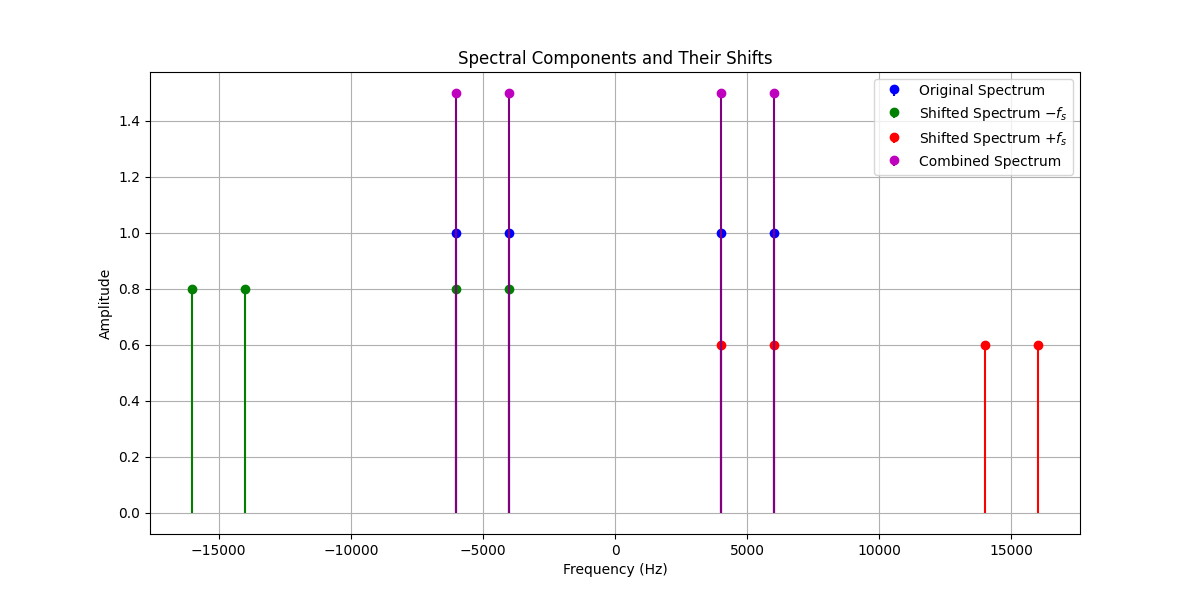
\includegraphics[width=0.8\textwidth]{fig/ex1_b_plot}
    \caption{Shifted spectra and resulting spectrum of $x[n]$}
    \label{fig:ex1b_spectrum}
\end{figure}

\subsection*{Conclusion}
The plot clearly shows how aliasing affects the spectrum of the sampled signal. Choosing an appropriate sampling frequency that is at least twice the highest frequency component of the signal (Nyquist rate) is essential to prevent aliasing and ensure signal integrity.
